% Student Number: 2240357068
% Student Name: Baturay KAFKAS
% EEE @ Hacettepe University

% My resource collection: https://github.com/kfksbtry/uni
% Circuits were set up in LTspice.

\documentclass{article}

\usepackage{graphicx}
\usepackage[top=25mm, bottom=25mm, left=25mm, right=25mm]{geometry}
\usepackage{amsmath}
\usepackage{moresize}
\usepackage{parskip}
\usepackage{float}
\usepackage{fancyhdr}
\usepackage{booktabs}
\usepackage{pgfplots}
\pgfplotsset{compat=1.18}
\usepackage{tikz}

\pagestyle{fancy}
\fancyhf{}
\fancyhead[R]{Baturay KAFKAS 2240357068 Electrical \& Electronics Engineering}

\rfoot{\thepage}
\renewcommand{\headrulewidth}{0pt} 
\renewcommand{\footrulewidth}{0pt}

\begin{document}

\large
\textit{This part of the experiment is prepared with Online LaTeX Editor Overleaf. Visit the website for the source here:}

\textbf{https://www.overleaf.com/read/xqcznrxycrxx\#b840fb}

\hrule

\vspace{1em}

\textbf{1. EXPERIMENT 5 - PRELIMINARY WORK}

\textbf{1.1} For the circuit given in \textit{Fig. 1}, sketch roughly the waveforms of $V_C(t)$ and $V_R(t)$.

\begin{figure}[H]
    \centering
    \includegraphics[width=0.75\linewidth]{chrome_Dtx92L2KLL.png}
\end{figure}

\textbf{Answer}: By a KCL equation for $0 < t < 1.32$ ms,

\[\frac{V_C-V_S}{R}=C\frac{dV_C}{dt}\implies\frac{dV_C}{dt}=\frac{V_C-V_S}{RC}\implies\frac{dV_C}{V_C-V_S}=\frac{dt}{RC}\]

\[\implies\int_{V_C(0)}^{V_C(t)}\frac{dx}{x-V_S}=\int_0^t\frac{d\tau}{RC}\implies-\ln\left|x-V_S\right|\bigg|_{x=V_C(0)}^{x=V_C(t)}=\frac{125000}{33}\tau\bigg|_{\tau=0}^{\tau=t}\]

\[\implies\ln\left(\frac{V_C(t)-V_S}{V_C(0)-V_S}\right)=-\frac{125000t}{33}\implies V_C(t)=V_S+(V_C(0)-V_S)e^{-125000t/33}\]

The voltage across the resistor is then 

\[V_R=V_S-V_C\implies(V_S-V_C(0))e^{-125000t/33}\]

One problem is that we need to know the value of $V_C(0)$, which is not given in the question. Assume that $V_C(0)=-5$ V. The voltages across the elements are

\[\left.\begin{array}{l}
V_C(t)=5-10e^{-125000t/3}\text{ V}\\
V_R(t)=10e^{-125000t/3}\text{ V}
\end{array}\right\}\:0< t< 1.32\text{ ms}\]

For $1.32\text{ ms}<t<2.64\text{ ms}$, the polarity of the source changes. Assume that the final voltages are attained, i.e., the difference in the voltage at $t=1.32$ ms and the final voltage is negligible. Therefore, the equations also change sign.

\[\left.\begin{array}{l}
V_C(t)=-5+10e^{-125000(t-1.32\text{ ms})/3}\text{ V}\\
V_R(t)=-10e^{-125000(t-1.32\text{ ms})/3}\text{ V}
\end{array}\right\}\:1.32\text{ ms}< t< 2.64\text{ ms}\]

Since $0< t<2.64\text{ ms}$ comprises one square wave, we can sketch the entire graph.

\begin{center}
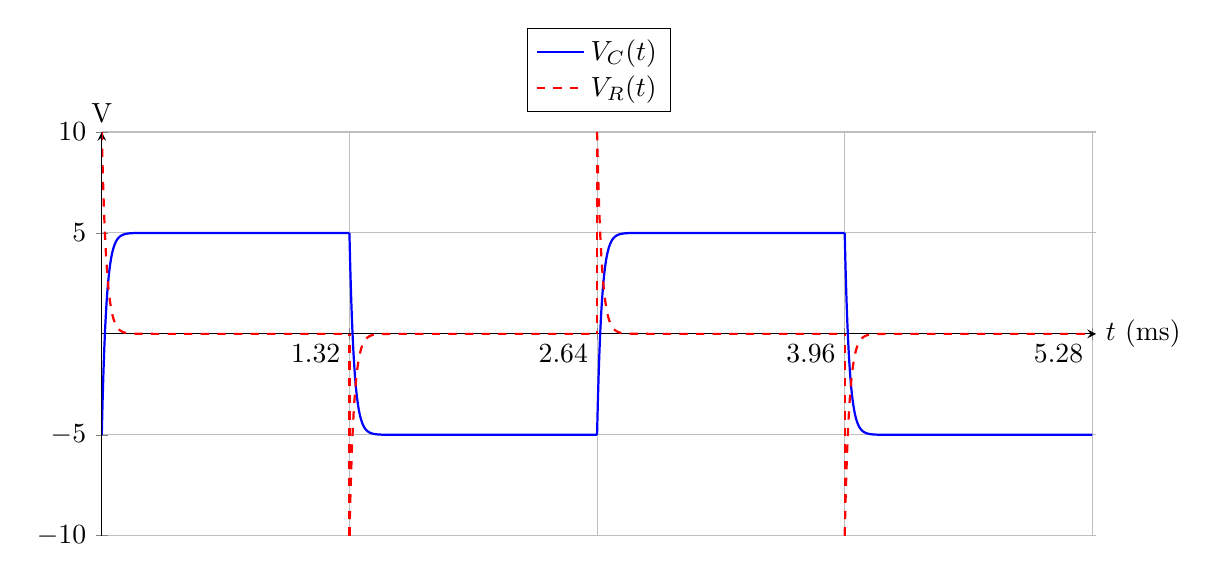
\begin{tikzpicture}
\begin{axis}[
    axis lines=center,
    width=10cm,
    height=5cm,
    xlabel={$t$ (ms)}, ylabel={V},
    xlabel style={at={(axis description cs:1,0.5)}, anchor=west}, % right end
    ylabel style={at={(axis description cs:0,1)}, anchor=south}, % above
    grid=both,
    xmin=0, xmax=5.3,
    domain=0:5.28,
    samples=300,
    legend style={at={(0.5,1.05)},anchor=south},
    scale=1.5,
    xtick={1.32,2.64,3.96,5.28},
    xticklabels=\empty
]

\addlegendimage{blue, thick}
\addlegendentry{$V_C(t)$}

\addlegendimage{red, thick, dashed}
\addlegendentry{$V_R(t)$}

% V_C(t)
\addplot[blue, thick, domain=0:1.32, forget plot] {5-10*exp(-125*x/3)};
\addplot[blue, thick, domain=1.32:2.64, forget plot] {-5+10*exp(-125*(x-1.32)/3)};
\addplot[blue, thick, domain=2.64:3.96, forget plot] {5-10*exp(-125*(x-2.64)/3)};
\addplot[blue, thick, domain=3.96:5.28, forget plot] {-5+10*exp(-125*(x-3.96)/3)};

% V_R(t) 
\addplot[red, thick, dashed, domain=0:1.32, forget plot] {10*exp(-125*x/3)};
\addplot[red, thick, dashed, domain=1.32:2.64, forget plot] {-10*exp(-125*(x-1.32)/3)};
\addplot[red, thick, dashed, domain=2.64:3.96, forget plot] {10*exp(-125*(x-2.64)/3)};
\addplot[red, thick, dashed, domain=3.96:5.28, forget plot] {-10*exp(-125*(x-3.96)/3)};

\node at (1.14,-1) {$1.32$};
\node at (2.46,-1) {$2.64$};
\node at (3.78,-1) {$3.96$};
\node at (5.1,-1) {$5.28$};

\draw[dashed, red, thick] (axis cs:1.32,-10) -- (axis cs:1.32,0);
\draw[dashed, red, thick] (axis cs:2.64,10) -- (axis cs:2.64,0);
\draw[dashed, red, thick] (axis cs:3.96,-10) -- (axis cs:3.96,0);

\end{axis}
\end{tikzpicture}
\end{center}
\end{document}